\subsection{Gestion de projet}

\subsubsection*{Méthode agile}
\addcontentsline{toc}{subsubsection}{Méthode Agile}

Lors de ce projet, nous avons, d'un commun accord entre nous 3 et Panorama Performance, décidé de mettre en place un système de management agile.\cite{Atlassian} En effet, le format de sprint\cite{Sprint} de 1 semaine s'adaptait parfaitement au concept de l'activ'Esaip.\\ 
\begin{figure}[h!]
    \centering
    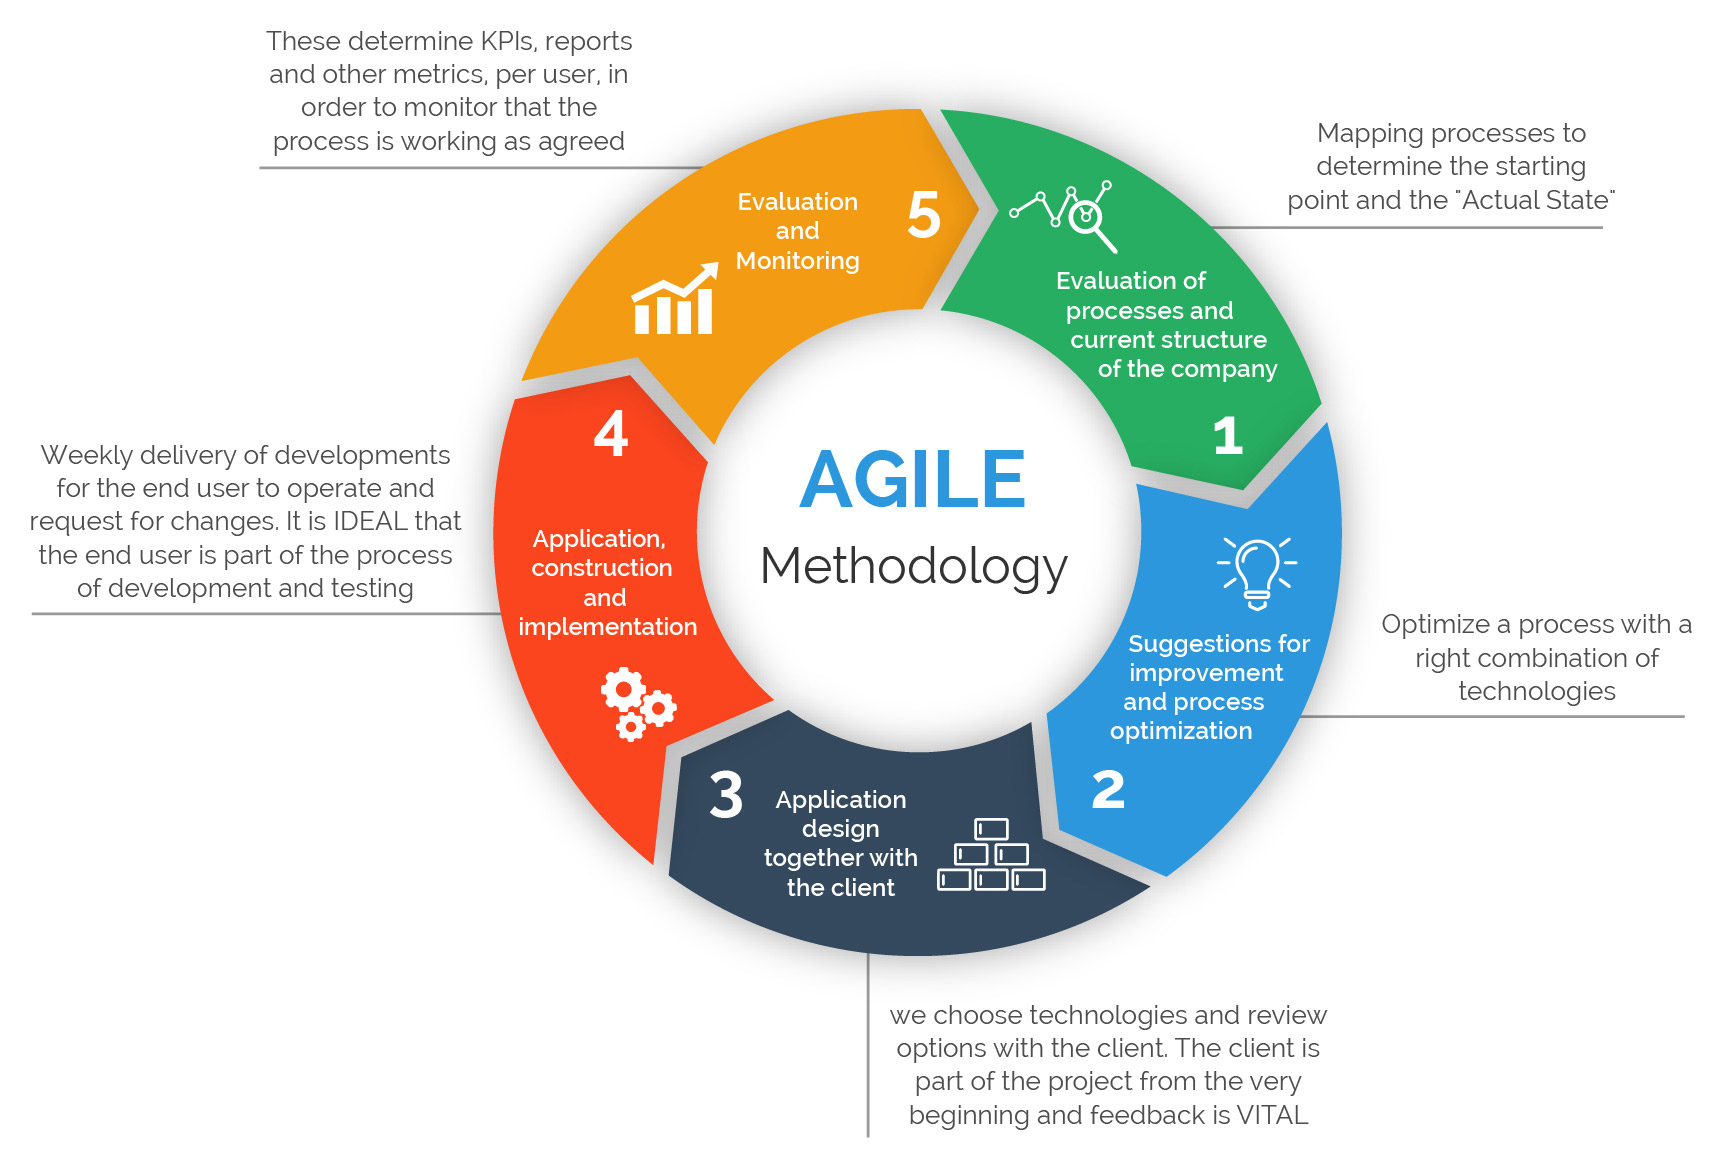
\includegraphics[scale=0.25]{img/agile.jpg}
    \caption{La méthodologie agile place le client au centre du projet.}
    \label{fig:Agile}
\end{figure}

Le management agile repose sur un système itératif ou les remarques du client sont prise en charge après chaque sprint pour apporter des modifications à la solution en cours de développement. 

\subsubsection*{Le client}
\addcontentsline{toc}{subsubsection}{Le client}
Dans le cadre de ce projet, nous avons considéré Panorama Performance comme le \textbf{client}, à chaque réunion de fin de sprint, nous faisions un bilan avec Mme. Oudard et/ou M. Lecointre pour rendre compte de l'avancement et prendre en compte leurs remarques pour le sprint suivant.\\

\subsubsection*{Le product owner}
\addcontentsline{toc}{subsubsection}{Le Product Owner}
Nous avons également désigné M.Oudard comme \textbf{product owner}\cite{ProductOwner} ; en tant que représentante de l'entreprise au sein de l'équipe, elle s'est chargée d'interpréter les besoins de l'entreprise pour en faire des outils fonctionnels.

M. Barbault s'est occupé de remplir le \textbf{backlog}\footnote{Planification hiérarchique des tâches} avec les \textbf{user stories}\footnote{Description simple d'un besoin du client} qu'elle nous communiquait.

\subsubsection*{Le scrum master}
\addcontentsline{toc}{subsubsection}{Le Scrum Master}


Dans la gestion de projet agile, le \textbf{scrum master}\cite{ScrumMaster} est un peu le coach de l'équipe ; il guide le projet dans la bonne direction sans pour autant être considéré comme un chef ou responsable. C'est également la représentation du management agile au sein de l'équipe : il aide à appliquer la méthodologie agile en donnant des conseils aux membres de l'équipe.

\begin{figure}[!h]
    \centering
    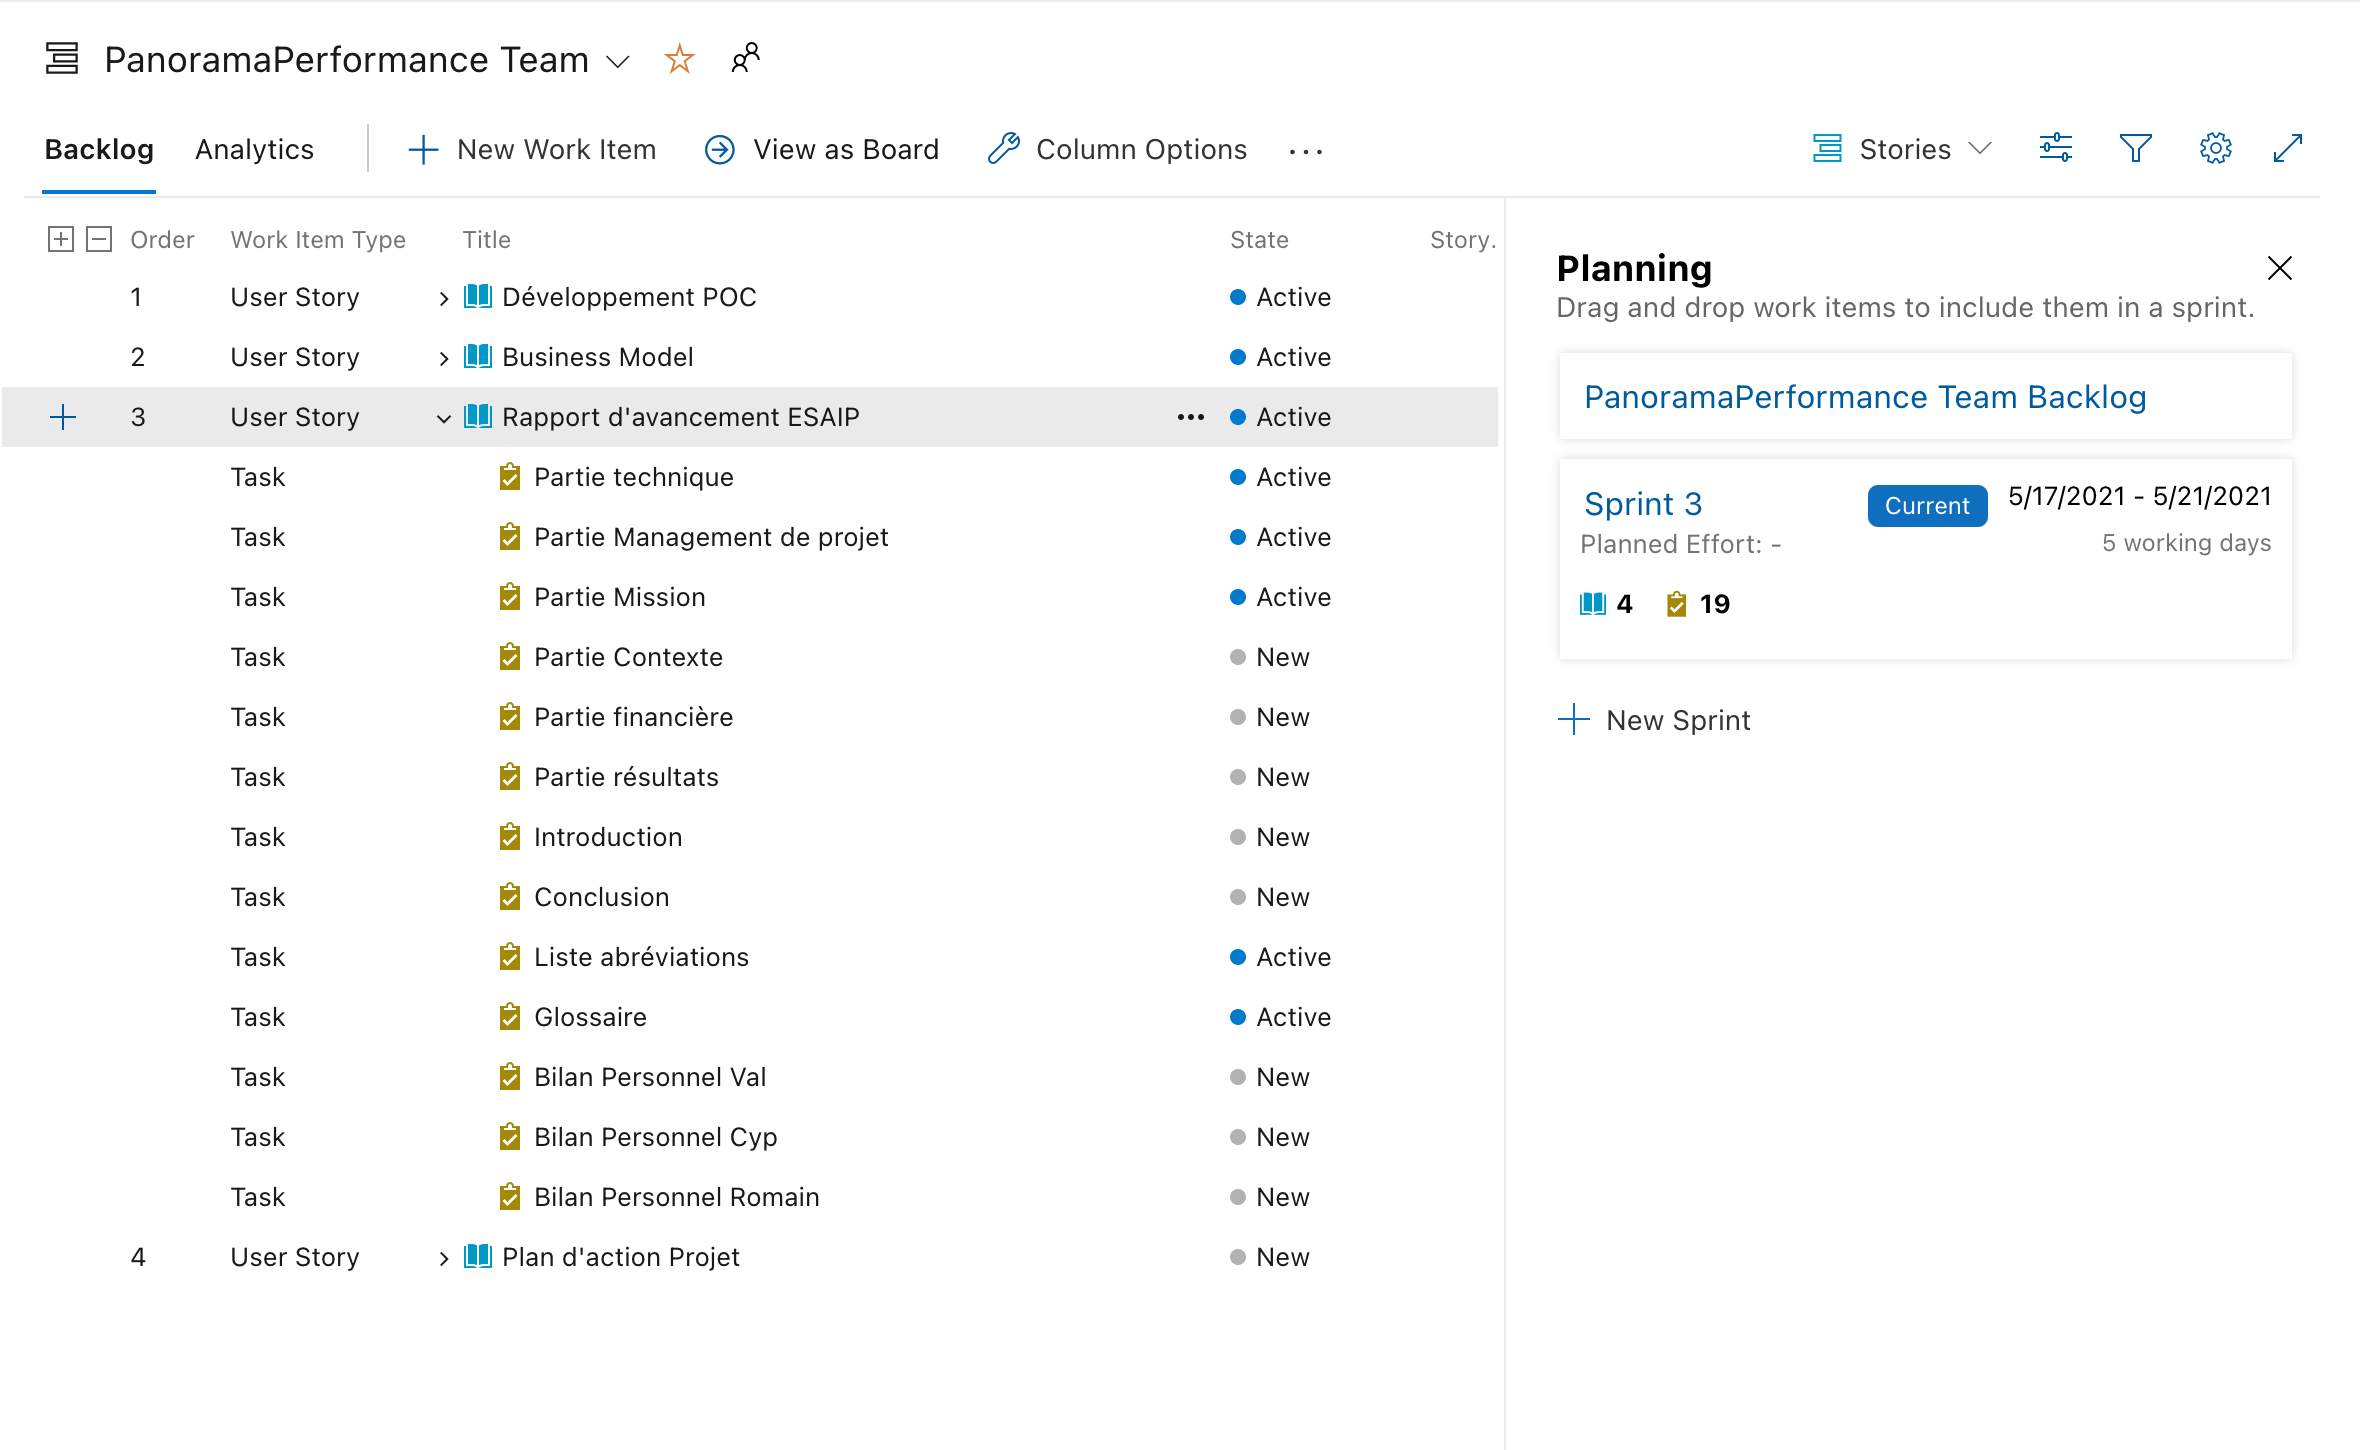
\includegraphics[scale=0.18]{img/backlog.png}
    \caption{Le backlog de notre projet lors du $3^{e}$ sprint}
    \label{fig:my_label}
\end{figure}

\subsubsection*{Déroulement d'un sprint}
\addcontentsline{toc}{subsubsection}{Déroulement d'un sprint}

Chacun des 5 sprints réalisés chez Panorama Performance s'est déroulé selon le même schéma : 
\begin{enumerate}
    \item Réunion de début de sprint
    \item un daily meeting par jour du sprint
    \item Réunion de bilan de sprint
\end{enumerate}

Le daily meeting est une réunion très courte (environ 15 minutes) durant laquelle chaque membre de l'équipe explique le travail qu'il a réalisé la veille, les problèmes qu'il a rencontré et ses objectifs pour la journée.\\
\hfill \\
La réunion de fin de sprint se déroule généralement avec l'équipe de Panorama Performance. C'est l'occasion de montrer les avancements de la semaine et voir avec Panorama Performance ce qui va ou ne va pas, de manière à le modifier pour le sprint suivant. Bien évidemment, notre tuteur ESAIP était convié à chacune de ces réunions.


\clearpage
\subsubsection*{Outils de gestion de projet}
\addcontentsline{toc}{subsubsection}{Outils de gestion de projet}

Pour nous aider dans notre gestion de projet, nous avons décidé d'utiliser différents outils :
\begin{itemize}
    \item Azure DevOps
    \item Slack
    \item Microsoft Teams
\end{itemize}

\textbf{Azure DevOps} possède le gros avantage de proposer à la fois un \textbf{repository GitHub\cite{GitHub}}\footnote{GitHub est un système de versionning de code} et l'ensemble des boards de management agile (Kanban board, backlog, sprint, \dots)\\

\begin{figure}[!h]
    \centering
    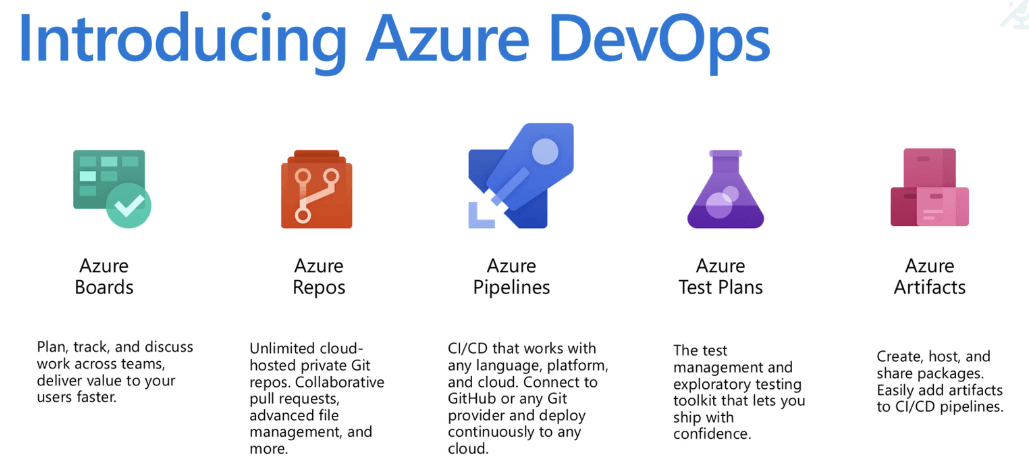
\includegraphics[scale=0.4]{img/azure.png}
    \caption{Azure DevOps, la solution de gestion de projet agile de Microsoft}
    \label{fig:my_label}
\end{figure}

C'est une plateforme très complète qui permet même d'associer à chaque \textbf{task}\footnote{Tâche en français. Fonctionnalité à implémenter/bug à résoudre dans le code} une \textbf{branche}\footnote{Une branche est une “copie" du code existant ; en réalisant une branche pour coder une nouvelle fonctionnalité il est facile de revenir en arrière en cas de problème} GitHub. De cette manière, le product owner n'a qu'à se charger de remplir le backlog avec l'ensemble des \textbf{user stories} et les tâches les composants ; puis l'équipe de développement créera une nouvelle branche de développement pour chacune de ces tâches. Lorsque le travail est terminé, la personne en charge du développement passe le code en validation (on appelle cela la \textbf{pull request}) ; de cette manière, le code est relu par les autres développeurs (dans notre cas, l'autre développeur), pour y déceler de possibles erreurs. Si les \textbf{reviewers} valident la modification, alors le nouveau code est ajouté au code pré-existant, sinon, le code est modifié jusqu'à entrer dans les critères.\\

\hfill \\
Si \textbf{Azure DevOps} était notre outil de gestion de projet par excellence, nous avions besoin d'un outil pour communiquer entre membres de l'équipe. Nous avons arrêté notre choix sur \textbf{Slack}\\

\begin{figure}[!h]
    \centering
    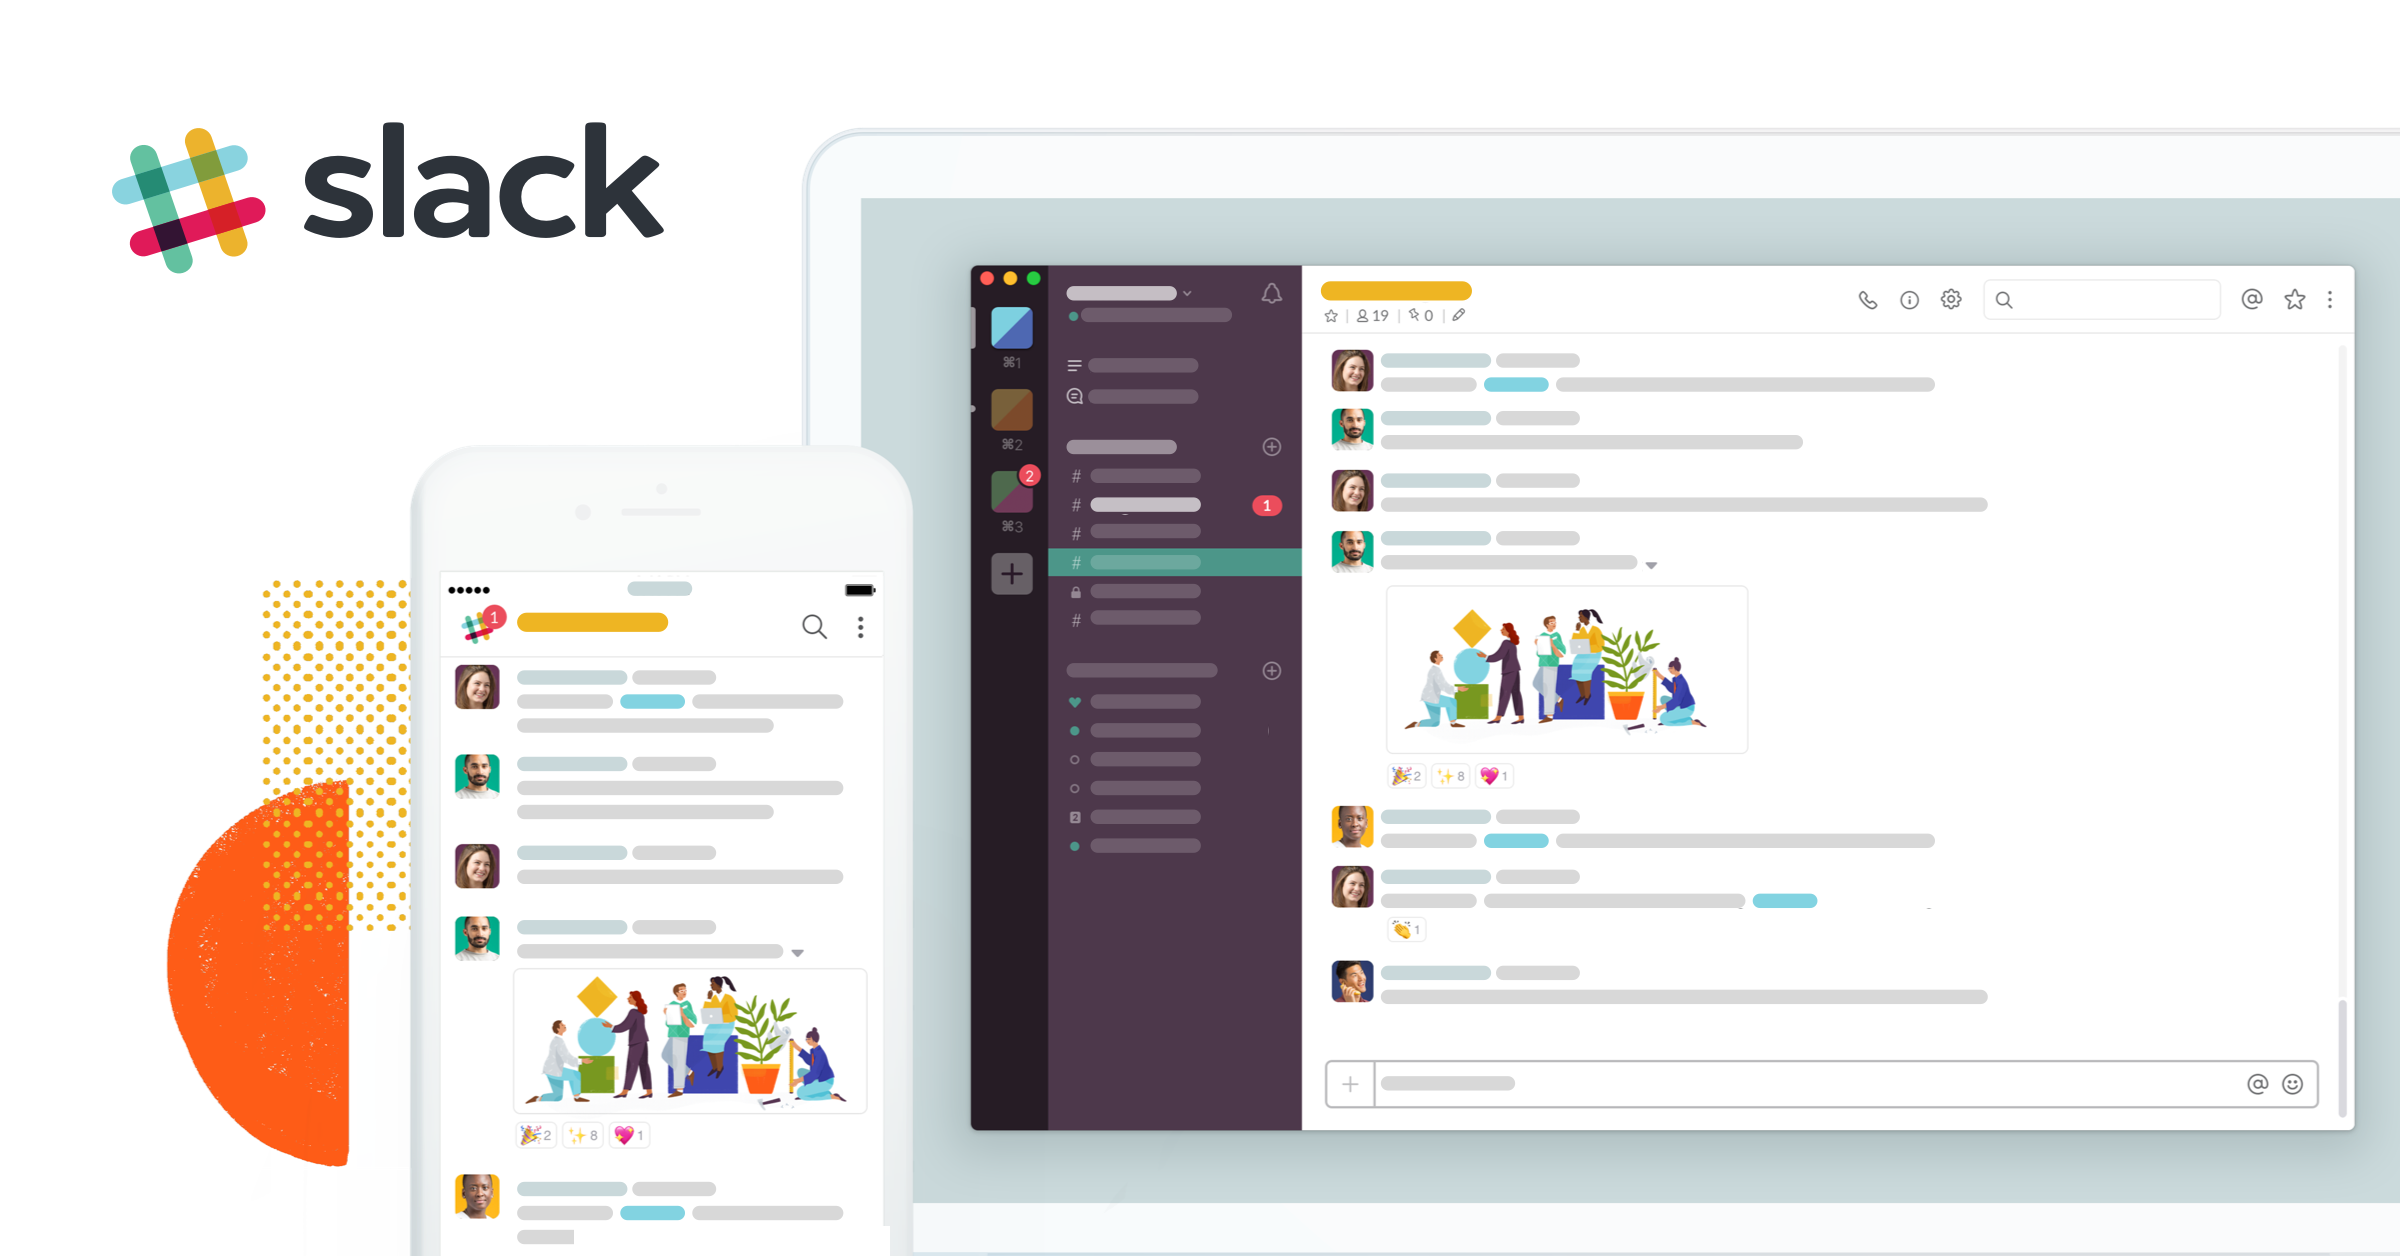
\includegraphics[scale=0.15]{img/slack.png}
    \caption{Slack, notre outil de communication interne}
    \label{fig:my_label}
\end{figure}

Slack facilite la communication entre équipes grâce à l'utilisation de canaux de discussion distincts en fonction du rôle de chacun au sein du projet. Ainsi, les non-développeurs n'ont pas besoin d'avoir accès aux canaux réservés au développement d'application tout comme seuls les membres du service comptabilité accéderont au canal qui leur est réservé.\\

Dans notre cas, M. \textsc{Lecointre} et Mme. \textsc{Oudard} n'avaient aucun intérêt à avoir les messages réservés au développement, cependant il était pratique d'avoir un canal dédié pour communiquer avec eux dans le cas où nous avions des questions à leur poser. M. \textsc{Albers} était évidemment lui aussi présent sur le \textbf{Slack} de manière à l'inclure dans notre projet et faciliter les préparations de réunion.\\

\begin{figure}[!h]
    \centering
    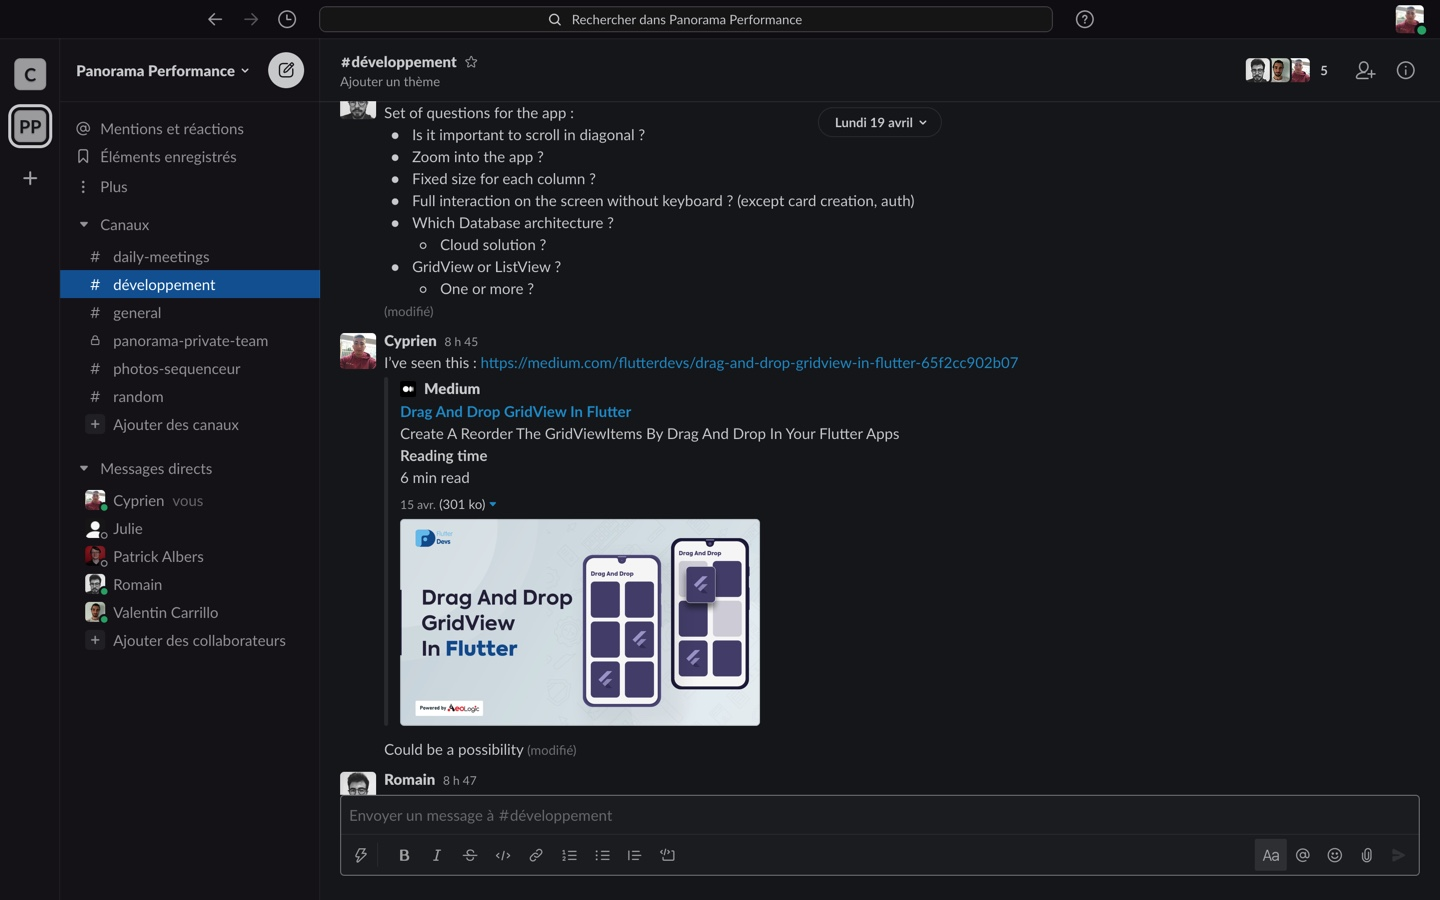
\includegraphics[scale=0.3]{img/screen_slack.jpeg}
    \caption{Le canal développement où nous discutions des choix techniques}
    \label{fig:my_label}
\end{figure}


Chaque daily meeting que nous avions tous les trois organisé était par exemple accessible par tous sur le canal \texttt{\#daily-meetings} sous forme d'un compte-rendu de réunion pdf.\\

Enfin, notre dernier outil de communication a été \textbf{Microsoft Teams}. Nous nous en sommes servis pour réaliser nos réunions avec M. Albers, tuteur au sein de l'ESAIP. Comme il nous est difficile de nous déplacer en ces temps de Covid, il nous a semblé préférable de réaliser les réunions d'avancement en visioconférence, et pour cela, Microsoft Teams est un outil fiable et nous permettant de partager nos écrans.

\begin{figure}[!h]
    \centering
    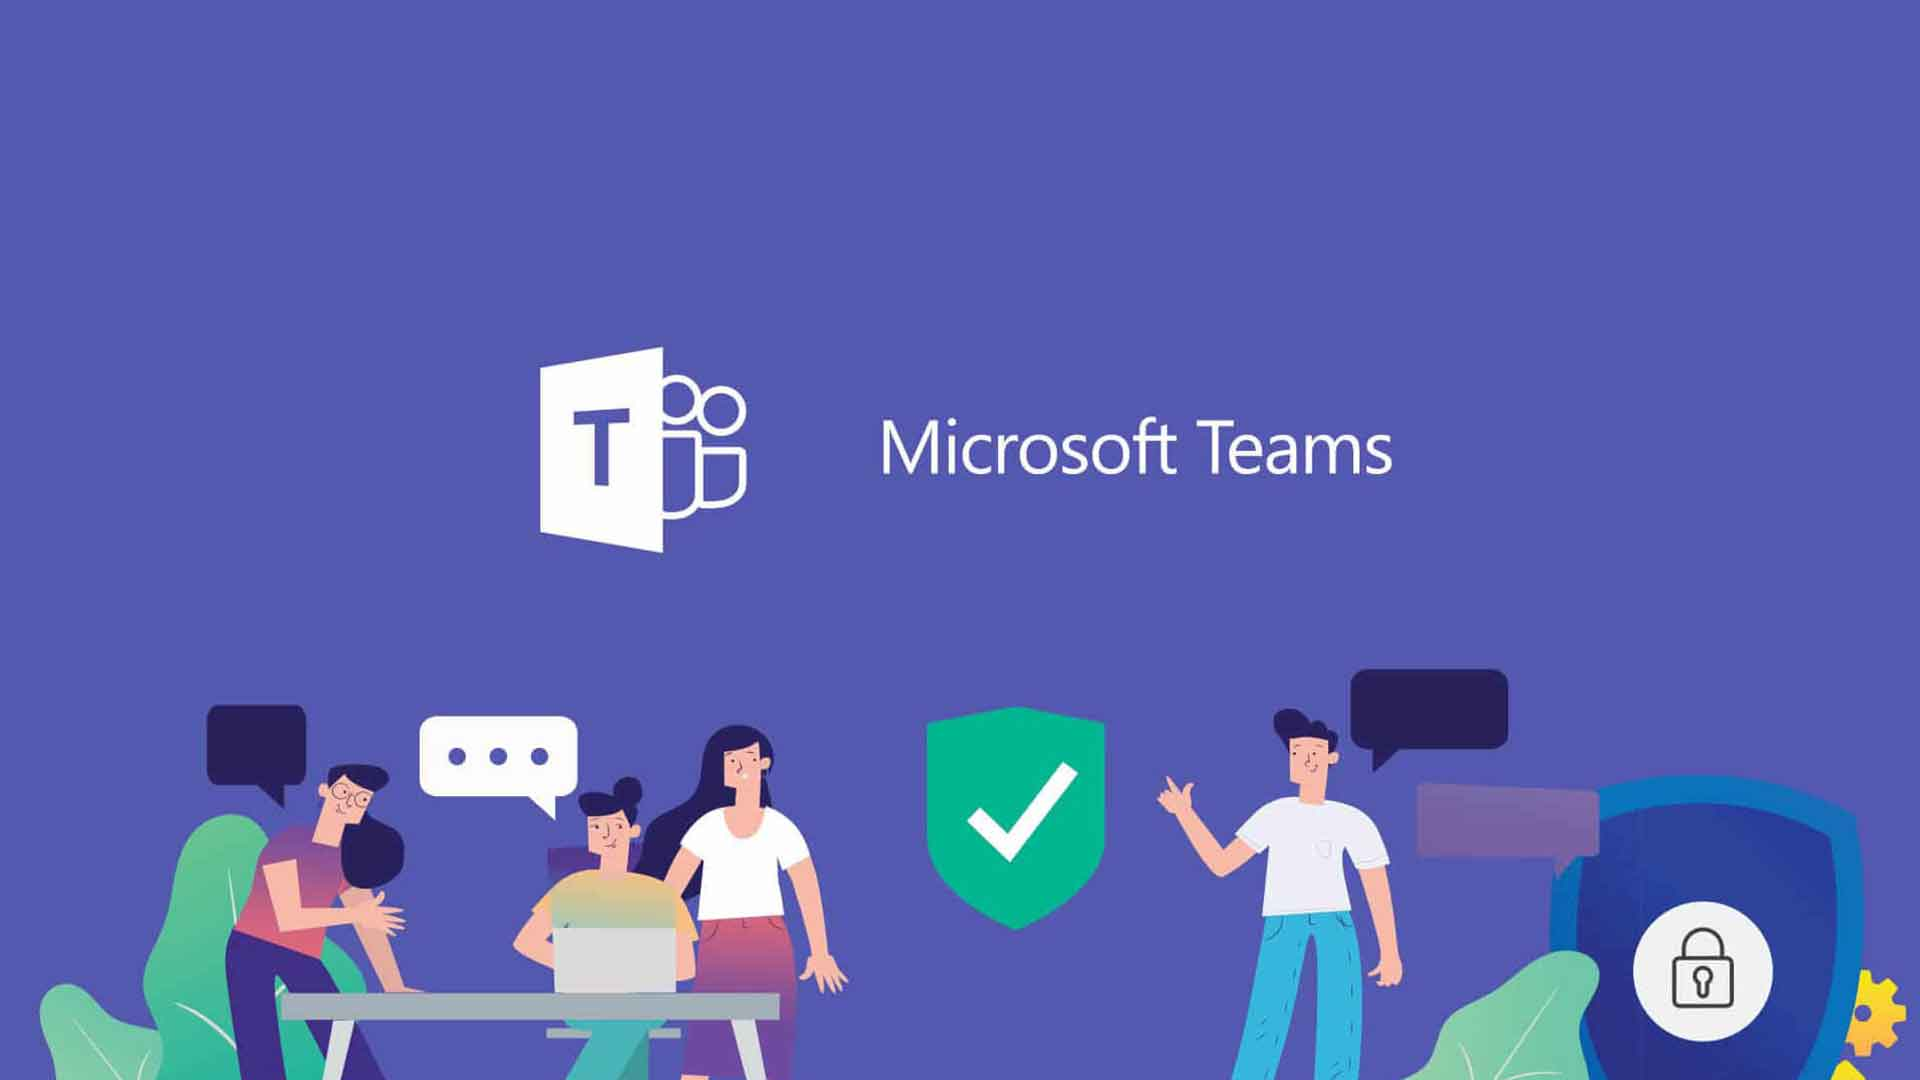
\includegraphics[scale=0.2]{img/teams.jpg}
    \caption{Microsoft Teams, notre outil de visioconférence}
    \label{fig:my_label}
\end{figure}

\subsubsection*{Pair Programming}
\addcontentsline{toc}{subsubsection}{Pair Programming}

Pour ce qui est de la partie programmation, nous avons voulu profiter de cette expérience en entreprise pour tenter un nouveau type de méthodologie de travail : \textbf{le pair programming}\cite{PairProgrammingCodementor}.\\

La technique de pair programming fonctionne de la manière suivante : un des deux développeurs écrit le code tout en l'expliquant, le second peut à tout moment proposer des améliorations ou sa vision du code. Au bout d'une vingtaine de minutes, les développeurs échangent de place pour que tout deux passent un temps égal devant le clavier. Le développeur qui n'est pas devant le clavier décide de l'axe directeur du code, quoi faire en premier, et quelles seront les étapes suivante\footnote{Bien évidemment, l'avis du second développeur est pris en compte, mais s'il faut trancher, ce n'est pas lui qui tranchera.}, un peu comme un copilote qui s'occuperait du GPS (voir figure \ref{fig:PairProgramming} ci-dessous)\\


\begin{figure}[h!]
    \centering
    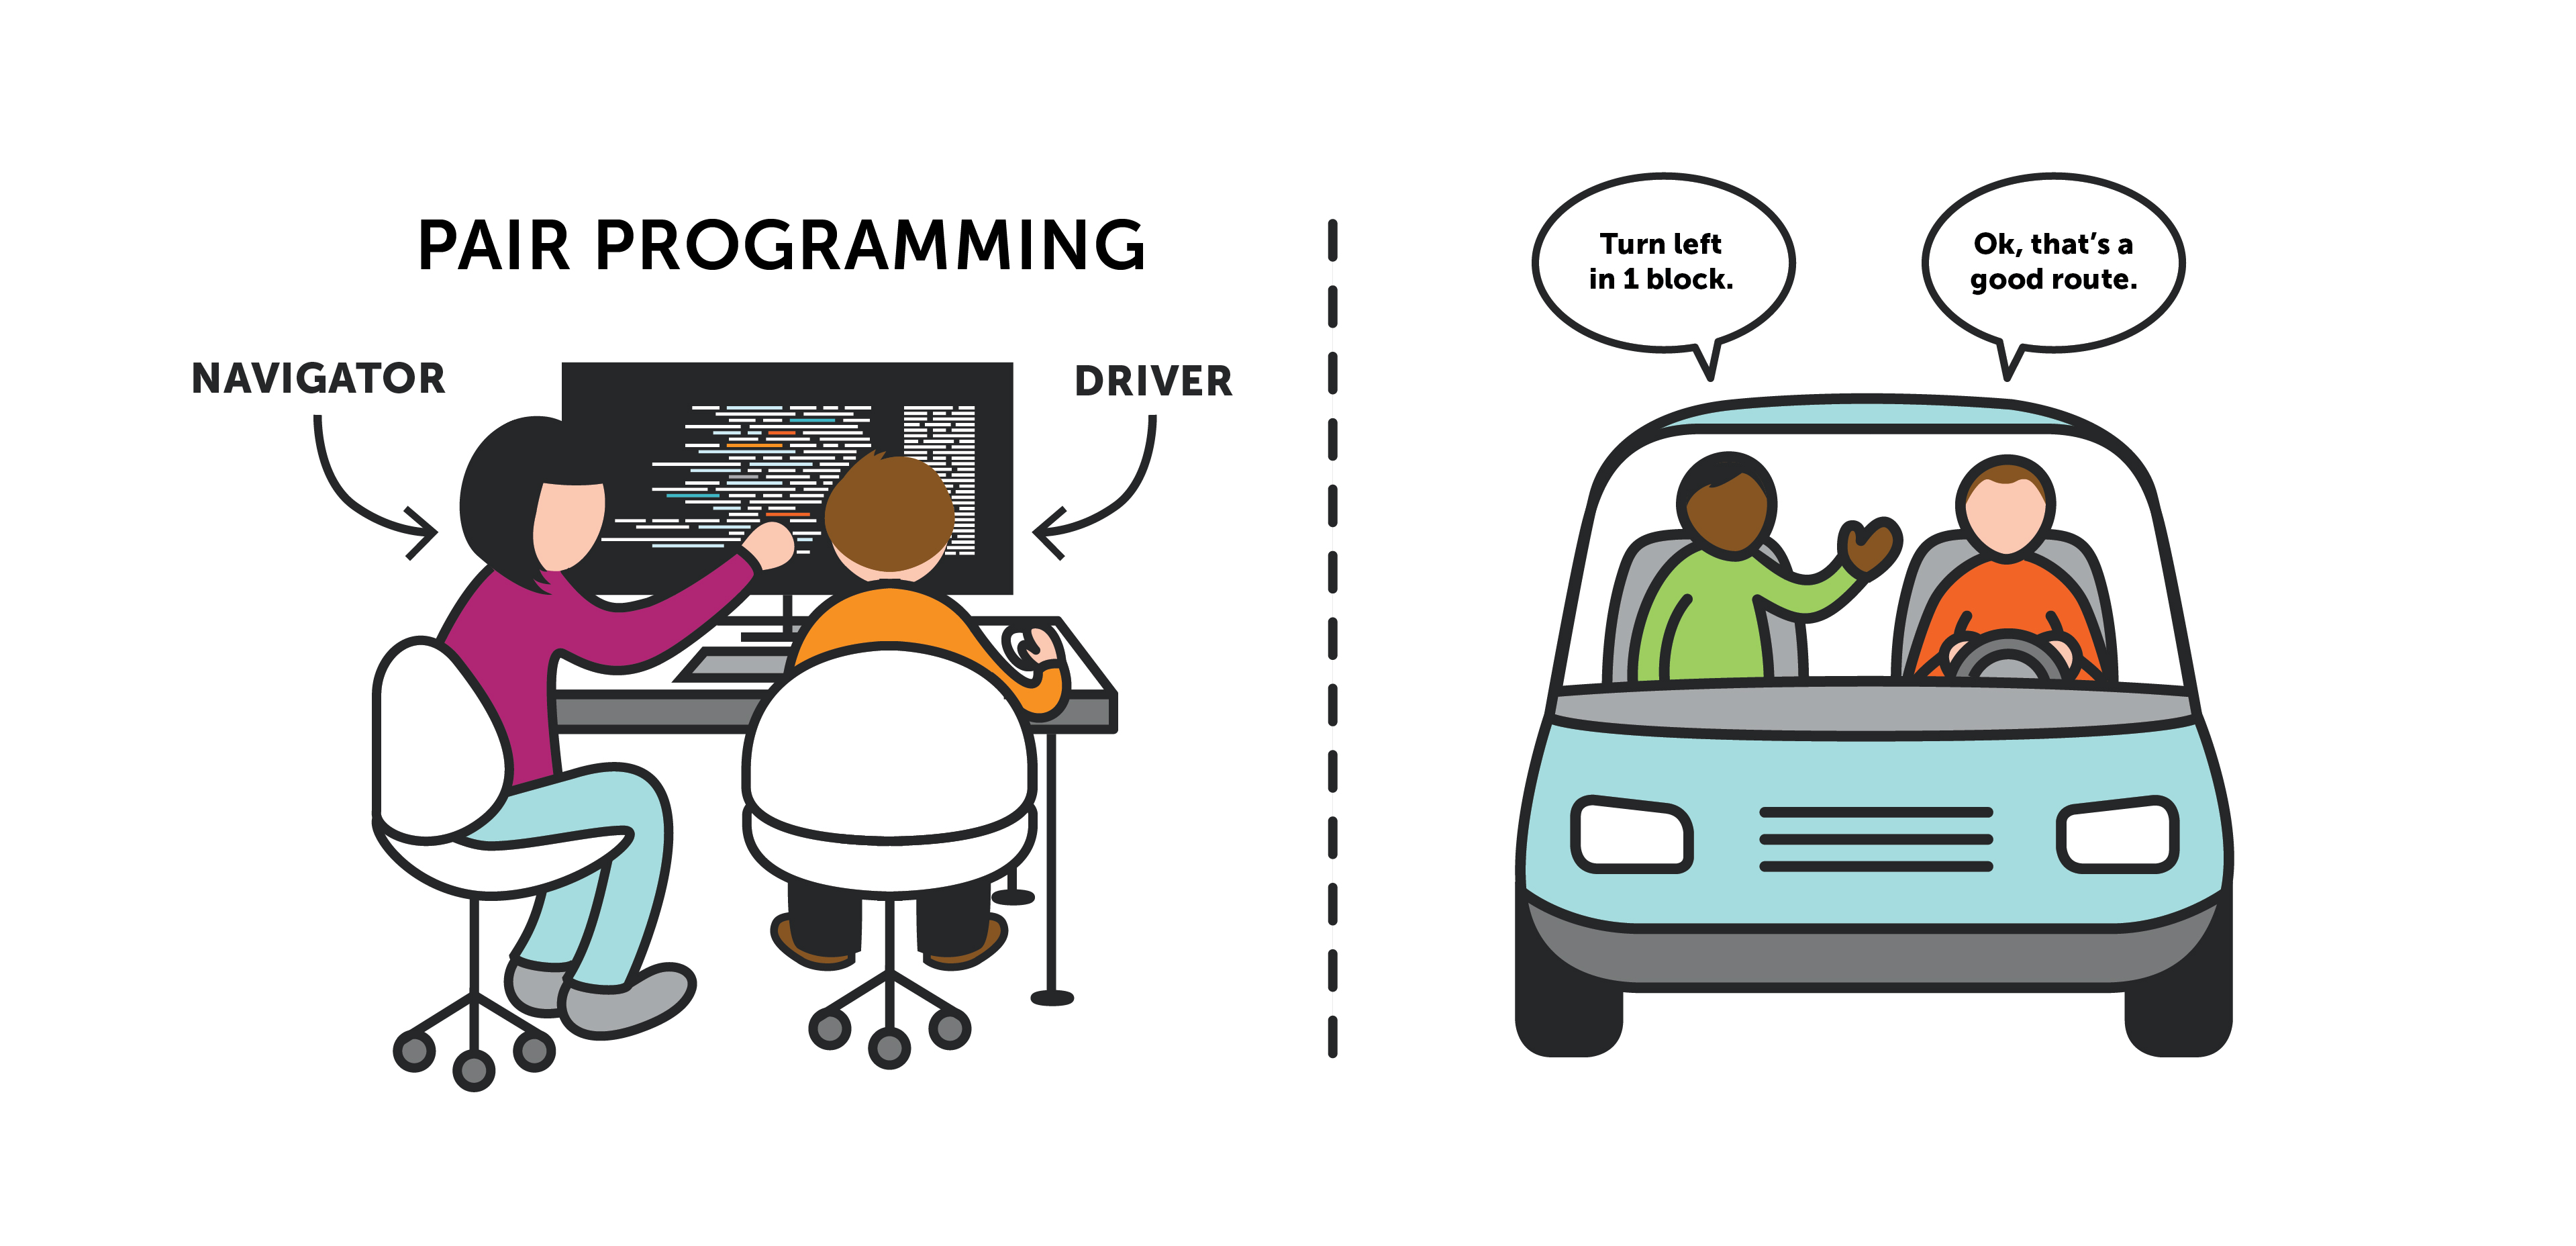
\includegraphics[scale=0.5]{img/pairprog.jpg}
    \caption{Le “pair programming", une technique de développement agile.}
    \label{fig:PairProgramming}
\end{figure}

L'intérêt d'une telle méthode est de produire un code de meilleure qualité en faisant travailler deux développeurs côte à côte ; de cette manière, deux approches sont confrontées dès la création du code et pas seulement dans la phase de debugging. La technique du pair programming est encore plus intéressante si l'on paire un développeur "senior" avec un "junior"\footnote{Entendre par là un développeur expérimenté dans le langage et un débutant}\\

Même si au premier abord, cette stratégie parait une perte de temps (deux fois moins de développeurs devant un clavier = deux fois moins de code, non ?), il n'en est en fait rien ! En effet, la partie gourmande en temps dans le développement d'applications est la réflexion ; écrire le code est très rapide une fois que les idées et la structure sont présents\footnote{Surtout de nos jours avec l'aide de \textbf{snippets} (auto-compléteur de code)}. Développer à deux permet d'éviter les erreurs d'étourderie ou les fausses bonnes idées, et ainsi gagner du temps de débugging. De plus, lorsque l'on travaille à deux, il y a une volonté de ne pas décevoir l'autre : on évite les distractions, les appels téléphoniques, on tape vite au clavier,\dots~Il y a quelqu'un pour nous aider à rester concentrés, ou lorsque l'on bute sur un problème de programmation. Enfin, d'après une étude menée en 2000, 96\% des développeurs ayant participé ont répondu mieux s'amuser lors du pair programming, et 95\% qu'il avaient plus confiance en leur code !~\cite{Williams00strengtheningthe}

\subsubsection*{Difficultés rencontrées et points d'améliorations}
\addcontentsline{toc}{subsubsection}{Difficultés rencontrées et points d'améliorations}

Bien que ce projet ne soit pas notre premier en terme de management de projet agile, nous sommes encore inexpérimentés sur certains concepts, et il nous arrive de ne pas respecter la mentalité \textsc{scrum} au pied de la lettre.\\

Ainsi, il n'était pas rare que la charge de travail que nous avions prévu lors du sprint planning ne soit pas suffisante, ou au contraire trop importante. Cela découle peut-être du fait que nous n'utilisions pas d'\textbf{indicateurs de performance} lors de notre projet. Il nous était donc impossible de calculer notre \textbf{vélocité}\footnote{En \textsc{scrum}, la vélocité est la charge de travail (en heure) que peut endurer l'équipe en un sprint.} ou d'afficher un \textbf{burndown chart}\footnote{Le burdown chart est un graphique affichant le nombre d'user stories en cours ou terminées ainsi que celles qui ont été créées durant le sprint} de qualité (voir figure \ref{fig:burndownChart}).\\

\begin{figure}[!h]
    \centering
    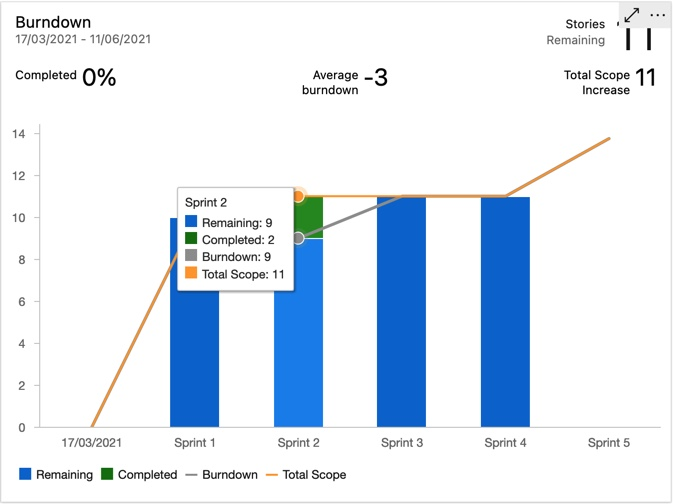
\includegraphics[scale=0.5]{img/burndown.jpeg}
    \caption{Le burdown chart}
    \label{fig:burndownChart}
\end{figure}

Pour combler le manque de charge de travail sur un sprint, nous étions dans l'obligation de modifier le sprint backlog, ce qui implique de rajouter des tâche au sprint en cours. Certes la team de développeurs se retrouvait avec du travail à réaliser, mais en contrepartie, il nous est arrivé de finir un sprint avec plus de travail à réaliser qu'à son début\footnote{Ce qui explique un burndown moyen négatif et une augmentation du scope\dots }

La taille de notre équipe est également un facteur négatif, la méthodologie \textsc{scrum} est plus complexe à mettre en place au sein de petites équipes, car le scrum master et/ou le product owner doivent alors doubler leur rôle en étant développeurs en même temps.\\

Mais il ne faut pas baisser les bras et rester agile ! Si ce projet n'a pas été mené à la perfection, les grandes lignes maîtresses du management agile ont été suivies et nous en avons beaucoup appris. À la manière agile, nous allons apprendre de nos erreurs et le prochain projet agile que nous mèneront n'en sera que meilleur.\\

Pour ce qui est du pair programming, cette première expérience s'avère concluante, même si toutes les directives n'ont pas étés tout le temps respectées à la règle. Par exemple, nous ne changions pas de rôle toutes les 20 minutes, ce qui provoqua un déséquilibre dans l'écriture de code que chacun de nous a réalisé. Cette pratique courante s'appelle \textbf{“Watch the Master"}\cite{enwiki:1023152145} et prend souvent place lorsqu'un développeur plus expérimenté prend place devant le clavier.


